% 图 3.13 自旋回波六阶段 3D 示意（NMR）
% (a) 平衡磁化沿 +z  (b) 90° 脉冲翻到 +y  (c)(d) 进动失相扇形展开
% (e) 180° 脉冲使扇形绕 x 翻转  (f) 重聚相沿 -y 形成回波
% 视角：z 上、y 右、x 向左下出纸；xy 面内虚线椭圆为进动轨迹
\documentclass[tikz,border=5pt]{standalone}
\usetikzlibrary{arrows.meta}
\usepackage{amsmath}
\usepackage{bm}
\usepackage{fontspec}
\setmainfont{Times New Roman}
\begin{document}
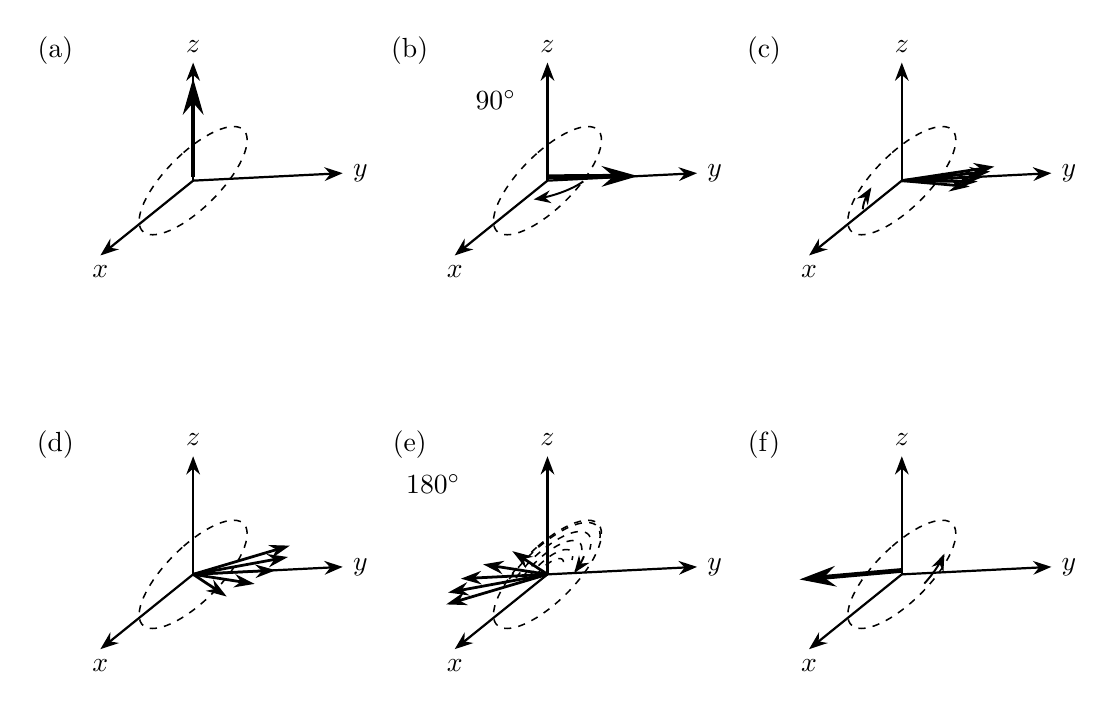
\begin{tikzpicture}[line width=0.8pt,>=Stealth,
  bar/.style={-{Stealth[length=4.6mm,width=2.6mm]},line width=1.7},
  far/.style={-{Stealth[length=2.6mm,width=1.7mm]},line width=1.0},
  ell/.style={dash pattern=on 2.6pt off 2.6pt,line width=0.55}]
% u(beta) = (sin b, cos b, 0)：b=0 沿 +y，向 +x 方向为进动正方向
\newcommand{\fanarrow}[2]{\draw[far] (0,0,0) -- ({#2*sin(#1)},{#2*cos(#1)},0);}
% xy 面内虚线椭圆（进动轨迹，半径 1.2）
\newcommand{\precellipse}{\draw[ell] plot[domain=0:360,samples=61]
  ({1.2*sin(\x)-0.744*cos(\x)},{0.072*sin(\x)-0.6*cos(\x)});}
% 坐标轴
\newcommand{\axes}{
  \draw[->] (0,0,0) -- (0,0,1.5) node[above]{$z$};
  \draw[->] (0,0,0) -- (0,1.9,0) node[right]{$y$};
  \draw[->] (0,0,0) -- (1.9,0,0) node[anchor=north]{$x$};}
% ---------- (a) ----------
\begin{scope}[shift={(0,5.0)},x={(-0.62cm,-0.50cm)},y={(1cm,0.05cm)},z={(0,1cm)}]
  \axes \precellipse
  \draw[bar] (0,0,0.05) -- (0,0,1.30);
\end{scope}
\node at (-1.75,6.65) {(a)};
% ---------- (b) ----------
\begin{scope}[shift={(4.5,5.0)},x={(-0.62cm,-0.50cm)},y={(1cm,0.05cm)},z={(0,1cm)}]
  \axes \precellipse
  \draw[bar] (0,0,0.05) -- (0,1.15,0);
  \draw[->,line width=0.7] plot[domain=8:78,samples=15]
    ({0.50*sin(\x)},{0.025*sin(\x)+0.50*cos(\x)});
\end{scope}
\node[anchor=south east,inner sep=1pt] at (4.15,5.85) {$90^\circ$};
\node at (4.5-1.75,6.65) {(b)};
% ---------- (c) 失相开始 ----------
\begin{scope}[shift={(9.0,5.0)},x={(-0.62cm,-0.50cm)},y={(1cm,0.05cm)},z={(0,1cm)}]
  \axes \precellipse
  \foreach \b in {-14,-7,0,7,14}{\fanarrow{\b}{1.05}}
  \draw[->,line width=0.7] plot[domain=12:50,samples=15]
    ({0.85*(-0.62*sin(\x)+cos(\x))},{0.85*(-0.5*sin(\x)+0.05*cos(\x))});
\end{scope}
\node at (9.0-1.75,6.65) {(c)};
% ---------- (d) 失相加剧 ----------
\begin{scope}[shift={(0,0)},x={(-0.62cm,-0.50cm)},y={(1cm,0.05cm)},z={(0,1cm)}]
  \axes \precellipse
  \foreach \b in {-38,-19,0,19,38}{\fanarrow{\b}{1.05}}
\end{scope}
\node at (-1.75,1.65) {(d)};
% ---------- (e) 180° 脉冲 ----------
\begin{scope}[shift={(4.5,0)},x={(-0.62cm,-0.50cm)},y={(1cm,0.05cm)},z={(0,1cm)}]
  \axes \precellipse
  \foreach \r in {0.35,0.55,0.75,0.95,1.15}{
    \draw[ell] plot[domain=55:205,samples=25]
      ({\r*(-0.62*sin(\x)+cos(\x))},{\r*(-0.5*sin(\x)+0.05*cos(\x))});}
  \foreach \b in {142,161,180,199,218}{\fanarrow{\b}{1.10}}
  \draw[->,line width=0.7] plot[domain=212:238,samples=12]
    ({0.85*(-0.62*sin(\x)+cos(\x))},{0.85*(-0.5*sin(\x)+0.05*cos(\x))});
\end{scope}
\node at (4.5-1.45,1.15) {$180^\circ$};
\node at (4.5-1.75,1.65) {(e)};
% ---------- (f) 回波重聚 ----------
\begin{scope}[shift={(9.0,0)},x={(-0.62cm,-0.50cm)},y={(1cm,0.05cm)},z={(0,1cm)}]
  \axes \precellipse
  \draw[bar] (0,0,0.05) -- (0,-1.30,0);
  \draw[->,line width=0.7] plot[domain=252:213,samples=15]
    ({1.0*(-0.62*sin(\x)+cos(\x))},{1.0*(-0.5*sin(\x)+0.05*cos(\x))});
\end{scope}
\node at (9.0-1.75,1.65) {(f)};
\end{tikzpicture}
\end{document}
